
% introduction
%  - vision/overview
%     - a decade from now robots will take the place along side humans and animals
%     - as companions, playmates, tutors, assistants
%     - there is a change in what we have to be, what we have to regard as peers to make this happen
%     - john henry vs robots
%  - why empathy for robots
%  - theory of life story
%  - description for rest of thesis


\chapter{Introduction}
\label{chap_intro}


   \begin{figure}[thpb]
      \centering
      
\includegraphics[width=4.6in]{figures/intro/tears_in_the_rain.png}
      \caption{Death of a replicant in the movie \textit{Blade Runner}}
      \label{fig_ec_story_no_story_lm}
   \end{figure}


What makes us human? This question is explored in the science fiction movie \textit{Blade Runner}. Set in a future-noir world against a backdrop of neon lit skyscrapers, we take on the persepctive of Deckard who is tasked with hunting down and killing replicants, an organic artificial humanoid. The replicants are assumed to be not human, a premise supported by their lack of moral rights. The movie suggests that what makes us human lies in the difference between the two. 

However, from this beginning, the movie systematically eliminates possible candidate differences: physical form, intelligence, motivation to survive, emotional experiences, and so on. The last ontological distinction is lost at the death of the lead replicant. In one of cinema's most memorable scenes, just before his death, the replicant says:

\begin{quotation}

``I've seen things you people wouldn't believe. Attack ships on fire off the shoulder of Orion. I watched C-beams glitter in the dark near the Tannh\"{a}user Gate. All those moments will be lost in time, like tears...in...rain. Time to die.''

\end{quotation}

As he dies, in an allegorical reference to the ascension of a soul, a dove leaves his hands and flies up into the light. What was lost at death was, in his own words, his unique experiences that we could only glimpse but not fully know. At that moment, we cannot help but feel moved by the death of the replicant \cite{rowlands_philosopher_end_universe}. The movie merges the ontological categories by having Deckard, who we had identified with, realizing after this scene that he might be a replicant himself \cite{mulhall_blade_runner}. 


Relating to and being emotionally engaged by life-stories of machines is a recurring theme in many science fiction works: \textit{2001: A Space Odyssey}, \textit{Ex Machina} and \textit{Otherspace}, to name a few. This thesis is an exploration of this theme.



\section{Research Question}

The main research question of this thesis is whether the implicit life-stories of a robot can invoke empathy for it. By implicit life-stories I mean the ability of the robot to experience the world we live in, to be transformed through that experience, and  to communicate the experience to us. By empathy for a robot, I mean understanding and experiencing the robot's perceived emotions as if they are our own. 

%
% Science fiction encourages us to imagine a world where we have companion robots that live alongside us and participate in our daily lives. Suspension of disblief is requested by placing this world in a distant future or in a galaxy far far away. However, this future isn't as foreign as these literary devices suggest. It is my belief that we are within a decade of having robots in our homes that can be companions, playmates, tutors and assistants. These robots may serve us, entertain us or teach us but most importantly we would find a sense of social other in them. One important aspect of relationships we have in our lives with either other humans or companion animals is that we feel empathy towards them. In this work, I propose one design critera for creating companion robots: giving robots an implicity life-story: the ability to experience the world, change through that experience and communicate it to us in a relatable way. I show that this ability encourages us to have empathy for the robot. 


\section{Why Empathy for Robots?}


   \begin{figure}[thpb]
      \centering
      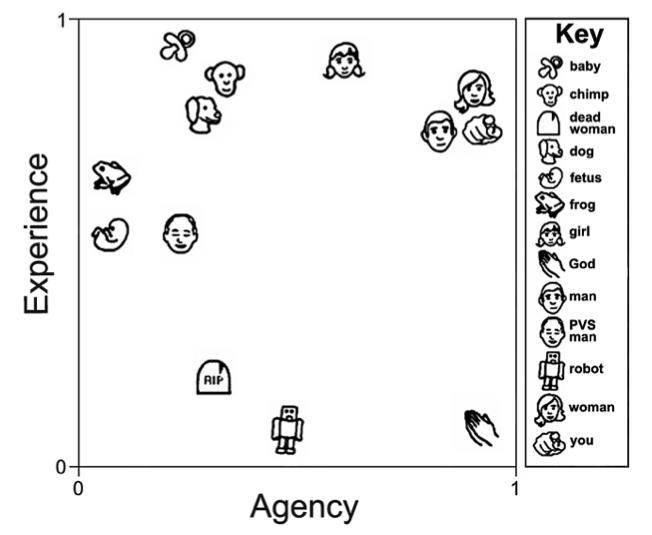
\includegraphics[width=4in]{figures/intro/gray_dimensions_mind.png}
      \caption{Gray et al.'s analysis of people's perception of minds of various character showed that robots are considered to be lacking in experience compared to other characters \cite{gray_dimensions_mind}}
      \label{fig_intro_gray}
   \end{figure}
   

Empathy for artificial agents has been proposed as a test of believability; that is to say, the greater the ability an agent has to invoke empathy, the more it is perceived  to be life-like \cite{paiva_empathic_virtual_agents}. A common conception of robots is that they do not have the capacity for emotions. Gray et al. examined people's perception of minds by asking participants to rank characters on various mental capacities (for example, out of a robot and a baby, which has greater capacity for pride, for telling right from wrong, etc.) and personal judgements (for example, who should be more deserving of blame if they were to cause harm to others) \cite{gray_dimensions_mind}.  Analysis of the responses showed that while robots were perceived to have agency that is comparable to other living entities, they were most lacking in affective experiences (See Figure \ref{fig_intro_gray}).  If we have empathy for robots, that is to say, we feel that we experience their emotions as if our own, then I argue that we implicitly believe that such robots have emotional experiences. Such capability could elevate the perception of robots to be closer to that of other living creatures. The process of bringing robots closer to us in our perception is, by construction, a pursuit of trying to understand who we are. 



   \begin{figure}[thpb]
      \centering
      
\includegraphics[width=4.6in]{figures/intro/paro_large.jpg}
      \caption{Residents at a retirement home find comfort in Paro, a therapeutic robotic seal\cite{nbcnews_paro}}
      \label{fig_intro_paro}
   \end{figure}
   

A second case for empathy towards robots is to create robots that can have roles similar to companion animals. There is wide evidence that companion animals have a beneficial effect on our physiological and psychological health. Interaction with companion animals has been shown to reduce loneliness, blood pressure, cholestorol, depression, anxiety, and stress \cite{walsh_human_animal_bond}. An important aspect of our relationship with animals is that we tend to feel empathy toward them. \cite{phillips_empathy_animals}. In addition, empathy toward companion animals can lead to greater empathy toward humans, which is a highly prosocial trait \cite{gullone_empathy_prosocial_pets}. It is worth exploring how to design robots to elicit empathy which could bring some of the benefits of companion animals to those who are unable to have them. 


%Empathy for artificial agents has been proposed as a test for believability ie. life-likeness \cite{paiva_empathic_veritual_agents}A common perception of robots is that they cannot have experiences of pain, pleasure or joy. This perception is related to personal judgements that robots are not deserving of moral rights or do not have a soul \cite{gray_dimensions_mind}. If we have empathy for robots, that is to say experience their emotions as if our then I argue that we implicity believe that such robots have emotional experiences. Such capability could elevate the perception of robots to be closer to that of other living creatures. This process of bringing the robot closer to us in perception is really a pursuit of trying to understand who we are by construction.


% robot as a tool for understanding who we are
% empathy for robots will inform robot's moral rights


\section{Implicit Life Stories}
\label{sec_intro_theory}

Living entities grow and change from experience over the course of their lives. Dautenhahn and Nehaniv described life as a complex story embedded in biology \cite{dautenhahn_nehaniv_alife}. Changes in morphology or behavior tell the story of the object. For example, consider encountering an one-eyed orange cat sunning itself on a wall. From that brief encounter, one extrapolates a checkered past of scuffles in alleyways and summers enjoying warmth. While I leave more to the reader's imagination, the point here is that through morphology and behavior, living creatures implicitly tell the stories of their lives. 

However, these stories are told imperfectly. They are not simple reproductions but rather underspecified ambiguous descriptions. Underspecificity, Gaver argued is a virtue, as it engages us as particpants \cite{gaver_ambiguity}. We become particpants in constructing the story. Ackermann wrote that viewers engage with objects by ``reconstructing them through the lens of their own interests and experiences.'' \cite{ackermann_experience_artifact} We color in the details of the stories using our own life-stories. We wince at the pain of the imagined fight that cost our orange cat his eye from past experience of our own pain. Empathy is generally defined as the ability to understand and feel what another feels \cite{decety_human_empathy}. If, through our own experience, we understand and are engaged by the experiences of another, then it stands to reason we would feel empathy for them. I posit that if we can build robots with implicit life-stories, we will feel empathy towards them. 

Based on the argument I outlined, I consider the following properties necessary for a robot to have an implicit life-story:

% By implicit-life stories I mean the ability of the robot to experience the world we live in, to be transformed through that experience, and  to communicate the experience to us. Empathy here means understanding and experiencing the robot's emotions as if they are our own.
\begin{itemize}
\item Autonomous agent: Robot can mean different things. For the purpose of implicit life-stories, all that is required is the robot is perceived to be capable of sensing and acting on the world driven by an internal process. This is necessary to be able to attribute experience to it. 
\item Perceptible change: The robot must change from experience. Without change, experience wouldn't leave an imprint on the robot. The change needs to be human perceptible so we would know of its existence and of the experience that caused it.
\item Relatable experience: The change to the robot must come from an experience that we could imagine ourselves having. A machine learning algorithm, learning to classify a dataset, is changing from experience but an experience we cannot share. Such an agent wouldn't qualify as having an implicit life-story by my definition. Embodiment and/or having human-like perception would make it easier for an agent to have a shareable experience.
\item Ambiguous Experience: As discussed earlier, the change to the robot must ambiguously reflect, or evoke, the experience it had. A video camera recording a movie is changing from a perceptual input that we could have. However, the perfect reproduction doesn't leave room for us to imagine a social model much less being able to put ourselves in its place. On the other hand given an input, the resulting change cannot be incomprehensible as that would preclude us from reconstructing the experience. 
\end{itemize}


Over the next few chapters, I share what I learned from building robots according to these ideas and testing my thesis with human subject studies. 


\section{Thesis Overview}

\hspace{7pt} Chapter \ref{chap_background}: I provide background for social robotics and empathy and describe the relationship of this work to these fields. I also note related work done on stories for artificial agents.

Chapter \ref{chap_lightbug}: I describe a minimal robot that I construct as a preliminary exploration
of implicit life-stories. Consider this as a thought experiment. 

Chapter \ref{chap_hexbug}: I test my thesis with a human robot interaction study where participants interact with a toy robot that has been given a fictional implicit life-story. After the interaction, the participants are asked to strike the robot. From measuring their hesitation to strike and through psychometric tests, I show that life-stories invoke empathy.

Chapter \ref{chap_design}: Based on the results from the initial human subject study, I build a sound robot that can have a life-story. In this chapter, I describe design considerations, the process of building the mechanical systems, and the architecture of the software necessary to animate the robot and to learn sounds. 

Chapter \ref{chap_pilot}: I then conduct pilot studies with human subjects to understand perception of the robot and to refine validation study design. I describe my experience of iterating on the design. 


Chapter \ref{chap_study}: I conduct controlled human subject study with both online and in person participants. I show that implicity life-stories create greater empathy for the new robot. I also find that empathy for robot can impact subsequent empathy for humans. 

Chapter \ref{chap_final}: I summarize my findings from my studies and my contributions to the field. I discuss ideas for extending this work and possible applications for such robot.



\section{Contribution}
As a preview of the final chapter, I submit these as my contributions:


\begin{itemize}
\item Proposed a new design element, implicit life-stories, for engendering empathy for social robots
\item Demonstrated empathy for robots with implicit life-stories through human robot interaction experiments across two different platforms
\item Designed and built a novel sound interaction social robot to embody and test these ideas
\item Demonstrated that the implicit life-stories can improve perception of social robot on animacy, anthropomorphism, likeability and intelligence measures
\item Showed that empathy for robot has an impact on subsequent empathy for humans. This is the first work to examine the connection between the two.
\item Open-sourced design and code for the new robot
\end{itemize}






%%%%%

%\section{In Popular Culture}
% - talk about recurring occurence of memories as the key part of movies about robots
% - talk about hitchbot and stories

% I am certainly not the first to suggest that a machine that can have experiences is emotionally meaningful to us. There are numerous references to such
% a notion in popular culture. In the movie, 2001 a space odyssey, there is a powerful scene where Dave is dismantaling Hal's memory bank. As
% Hal looses his memory he regresses and starts to recite nursery rhymes. Watching the scene there is a sense of a loss of a sentient being and one cannot
% help but feel sad for Hal. 

% In another movie, Blade Runner, just before death during poignant scene, the main antagonist, Roy Batty, laments that all his unique experiences will be lost.
% In an allegorical moment a dove escapes from his hands and flies off into the sky. This is regarded as Cinema's top 100 memorable scenes. The allegory refers
% to the flight of his soul. The corporal body remains and in the case of robots, believed to perfectly resuable, but the memories are gone.  These
% reflect this sense that it is the memory and the experience that matters. One sees motif repeated in science fiction but also in real life. 

% When the canadian hitch-hiking robot, HitchBot, got violently dismembered and tossed into a garbage dump, there was an outpouring of sympathy. 


% One of science fiction film's most dramatic moments is the death scene of an android, Roy Batty, in the movie Blade Runner. The movie is set in a
% world inhabited by humans and also androids. The androids while appearing human and having intelligence and even capacity for emotions are regarded
% as distinct from humans and impassionately hunted down and killed. However, in a climatic scene, the lead android is about to pass away and before
% pasisng he recounts his experiences in a famous soliliquoy: ``I have seen things you people wouldn't believe... c-beams glitter in the darkness...
% all these will be lost in time...'' It's a transforming moment. At that final brief moment, Roy seems human and one feels sad for him. THe crew 
% reportedly wept at the scene. 

% What I find fascinating here is that final humanizing moment, what the character puts forward is his story. This is the final bit that makes him relatable
% and invokes empathy for him. 


% Have you seen the movie Blade Runner? The science fiction movie is set in a world populated by humans and androids that look exactly human and behave almost similarily to the point that it is difficult to tell them apart from humans. A cenral theme of rhte movie is trying to understand how teh androids are not human or that is to say that what makes us different from robots. Do androids have a soul or are they just amchines? Near the end of the movie, there is a climatic scene, one of the most memorable ones in cinema, where the lead android, the antagonist dies. As he dies he says " I have seen all these things, you people wouldn't believe...." And at his death, a pigeon flies into the sky in allegorical scene as if his soul is leaving the body. What I find poignant is what is lost are the memories and experiences of this android described ambiguously in this beautiful solilquoy. The soul of the machine are these experiences. 

% This is a theme that is repeated in many science fiction descriptions of fictional AI: 2001 a space odyssey, ex machina, other space. Perhaps the anime that we seek to imbibe robots with is in the ability of the robots to create life-stories. 

